\documentclass[12pt]{beamer}

\usepackage{algorithm}
\usepackage[noend]{algorithmic}
\usepackage[english]{babel}
\usepackage[utf8]{inputenc}
\usepackage{minted}

\usetheme{Copenhagen}
\setbeamertemplate{navigation symbols}{}
\setbeamertemplate{bibliography entry title}{}
\setbeamertemplate{bibliography entry location}{}
\setbeamertemplate{bibliography entry note}{}
\setbeamertemplate{footline}[frame number]

\newtheorem{claim}{Claim}
\newtheorem{observation}{Observation}

\title{
  \texttt{import requests \&\&}\\
  \texttt{import threading} \(\implies\)\\
  \texttt{import scrapy}
}
\author[Jacopo Notarstefano]{
  Jacopo Notarstefano\\
  \texttt{jacopo [at] nabla.com}
}
\date{September 10th, 2019}

\begin{document}
  \begin{frame}[plain]
    \titlepage
  \end{frame}

  \begin{frame}{The Problem}
    Let's suppose that someone asks you to scrape a website containing a
    certain collection of \(N\) articles (\(N \approx 10^4\)), where each
    article is a webpage roughly one megabyte in size.

    \vspace{0.5cm}

    You start thinking about using the Python package \texttt{requests},
    perhaps paired for performance reasons with the \texttt{threading}
    portion of the standard library, but then you start worrying about
    the GIL...
  \end{frame}

  \begin{frame}{The Solution}
    \begin{figure}
      \centering
      \fbox{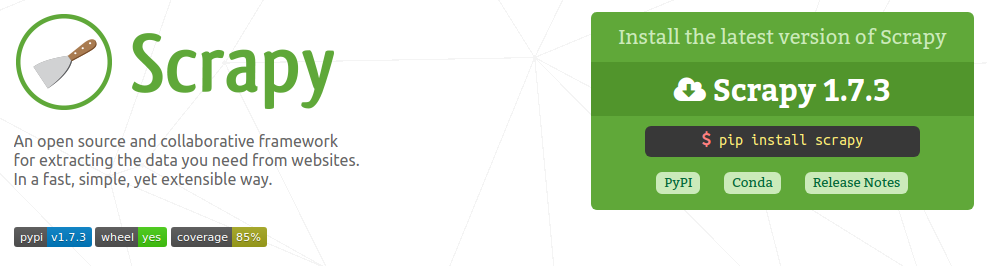
\includegraphics[width=\textwidth]{tex/img/scrapy}}
    \end{figure}
  \end{frame}

  \begin{frame}{A Claim}
    \begin{claim}[Notarstefano, 2019]
      Any piece of code that uses both \textup{\texttt{requests}} and
      \textup{\texttt{threading}} should instead be a \textup{\texttt{scrapy}}
      spider.
    \end{claim}
  \end{frame}

  \begin{frame}{A First \texttt{scrapy} Spider}
    \inputminted[fontsize=\scriptsize]{python}{tex/src/blogspider.py}

    \vspace{0.5cm}

    We can invoke it with \texttt{scrapy runspider blogspider}.
  \end{frame}

  \begin{frame}{A First \texttt{scrapy} Project}
    We can bootstrap a new \texttt{scrapy} project by running the command
    \texttt{scrapy startproject newproject}. We will end up with the following
    directory structure:

    \vspace{0.5cm}

    \inputminted[fontsize=\scriptsize]{shell-session}{tex/src/tree}
  \end{frame}

  \begin{frame}{Data Flow in \texttt{scrapy}}
    \begin{figure}
      \centering
      \fbox{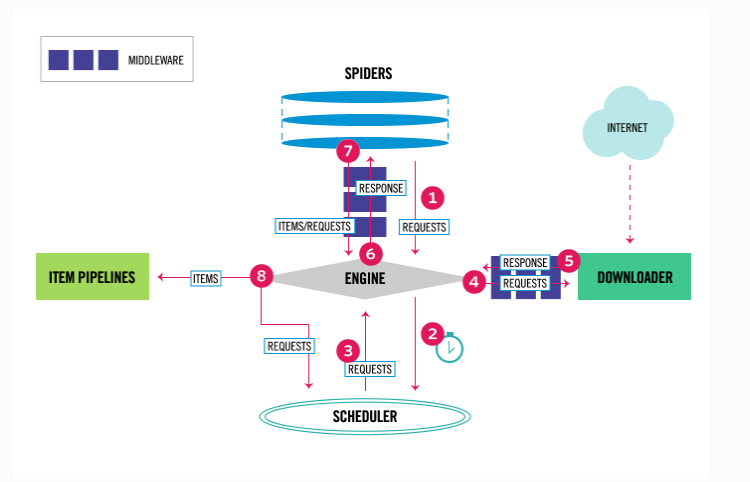
\includegraphics[width=\textwidth]{tex/img/architecture}}
    \end{figure}
  \end{frame}

  \begin{frame}{Items in \texttt{scrapy}}
    \inputminted[fontsize=\scriptsize]{python}{tex/src/productitem.py}

    \vspace{0.5cm}

    Item instances are simple containers used to collect scraped data.
    They also provide a way to specify how data should be serialized.
  \end{frame}

  \begin{frame}{Pipelines in \texttt{scrapy}, 1/2}
    \inputminted[fontsize=\scriptsize]{python}{tex/src/pricepipeline.py}

    \vspace{0.5cm}

    Item Pipelines provide a way of specifying linear workflows that Item
    instances will go through before being emitted or eventually discarded.
  \end{frame}

  \begin{frame}{Pipelines in \texttt{scrapy}, 2/2}
    \inputminted[fontsize=\scriptsize]{python}{tex/src/itempipelines.py}

    \vspace{0.5cm}

    Item Pipelines are configured by modifying the appropriate variable
    in the \texttt{settings.py} file, alongside their priority.

    \vspace{0.5cm}

    Note however that you typically won't need to define a
    \texttt{JsonWriterPipeline} as in the example, because you can use the
    predefined Feed Exporter for JSON.
  \end{frame}

  \begin{frame}{Middlewares in \texttt{scrapy}}
    There are two kinds of Middlewares in \texttt{scrapy}: the ones that
    intercept Request and Responses of Spiders and the ones that do the same
    for Downloaders.

    \vspace{0.5cm}

    They are allowed to do pretty much anything, including discarding the
    Request or generating multiple Responses. Let's see some examples from the
    documentation.

    \vspace{0.5cm}

    Once again, they are configured by modifying the
    \texttt{SPIDER\_MIDDLEWARES} and \texttt{DOWNLOADER\_MIDDLEWARES}
    respectively in the \texttt{settings.py} file.
  \end{frame}

  \begin{frame}{Spiders in \texttt{scrapy}}
    Finally, Spider classes should ideally contain only the logic that deals
    with extracting the relevant information from the downloaded page into
    Items, or generating more Requests for other pages.

    \vspace{0.5cm}

    \begin{observation}
      It's very easy to fall into the trap of putting all the logic in the
      Spider class. Instead, HTTP-level logic belongs to Downloader
      Middlewares, while business logic belongs to Pipelines.
    \end{observation}
  \end{frame}

  \begin{frame}{Developing and Debugging Spiders}
    The \texttt{scrapy shell} command is invaluable when developing and
    debugging.  Let's see it in a live example.
  \end{frame}
\end{document}
